\documentclass{standalone}
%\usetikzlibrary{...}
\usepackage{tikz}
\begin{document}
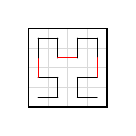
\begin{tikzpicture}
\tikzstyle{helperline} = [lightgray!60!white, line width=0.1mm] 
\draw[line cap=round][helperline]  (0.25,1.0) -- (0.25,-0.0);
\draw[line cap=round][helperline] (0.5,1.0) -- (0.5,-0.0);
\draw[line cap=round][helperline] (0.75,1.0) -- (0.75,-0.0);
\draw[line cap=round][helperline] (-0.0,0.75) -- (1.0,0.75);
\draw[line cap=round][helperline] (-0.0,0.5) -- (1.0,0.5);
\draw[line cap=round][helperline] (-0.0,0.25) -- (1.0,0.25);
\draw[line cap=round]  (0,1) rectangle (1,0);
\draw[line cap=round] (0.125, 0.125) -- (0.375, 0.125);
\draw[line cap=round] (0.375, 0.125) -- (0.375, 0.375);
\draw[line cap=round] (0.375, 0.375) -- (0.125, 0.375);
\draw[line cap=round,red] (0.125, 0.375) -- (0.125, 0.625);
\draw[line cap=round] (0.125, 0.625) -- (0.125, 0.875);
\draw[line cap=round] (0.125, 0.875) -- (0.375, 0.875);
\draw[line cap=round] (0.375, 0.875) -- (0.375, 0.625);
\draw[line cap=round,red] (0.375, 0.625) -- (0.625, 0.625);
\draw[line cap=round] (0.625, 0.625) -- (0.625, 0.875);
\draw[line cap=round] (0.625, 0.875) -- (0.875, 0.875);
\draw[line cap=round] (0.875, 0.875) -- (0.875, 0.625);
\draw[line cap=round,red] (0.875, 0.625) -- (0.875, 0.375);
\draw[line cap=round] (0.875, 0.375) -- (0.625, 0.375);
\draw[line cap=round] (0.625, 0.375) -- (0.625, 0.125);
\draw[line cap=round] (0.625, 0.125) -- (0.875, 0.125);
\end{tikzpicture}
\end{document}
